\documentclass[twocolumn]{article}
\usepackage{amsmath}
\usepackage{graphicx}
\usepackage{subcaption}

%borders
\usepackage{float}
\floatstyle{boxed}
\restylefloat{figure}


\title{Modularizing Street Map Generation \\
    \vspace{8pt} \large An Adventure in Tensors}
\author{William Clarkson \and Marcella Hastings \and Nathaniel Tenczar}
\date{\today}

\newcommand{\sqmat}[4]{\ensuremath{
    \left(\begin{array}{cc}
        #1 & #2 \\
        #3 & #4
    \end{array}\right)}}
\newcommand{\mkvec}[2]{\ensuremath{
    \left(\begin{array}{c}
        #1 \\
        #2 \\
    \end{array}\right)}}
\newcommand{\pt}{\textbf{p}}
\newcommand{\todo}[1]{\begin{center}\fbox{\parbox{150pt}{#1}}\end{center}}
\def \cpp {C\nolinebreak[4]\hspace{-.05em}\raisebox{.4ex}{\tiny\bf ++}~}

\begin{document}
\maketitle

\begin{abstract}
This paper addresses the issue of creating modular, extensible code given an
existing solution to a problem, namely, interactively modeling large street
networks. We describe a functional implementation of a framework that allows
users to create a realistic street network over an empty domain, based on the
techniques described in \textit{Interactive Procedural Street Modelling}
\cite{chen}. In particular, we were able to express the underlying mathematics
more intuitively and clearly than is possible in an imperative language.
\end{abstract}

\section{Introduction}
Visual artists often face the time-consuming task of generating extensive,
realistic scenes by hand for movies and video games. However, the apparent
randomness found in systems like street layouts can be modelled effectively
with a variety of mathematical algorithms, giving rise to the growing field of
procedural generation. In this paper we will discuss an algorithm using tensor
fields, from \cite{chen}, to generate realistic city street maps. To facilitate
the generation of aesthetically pleasing maps which fit an artist's
requirements, we implement a simple system of user-specified constraints to
allow the user to shape the resulting street map to fit their needs.

\section{Existing Work}
\textit{Interactive Procedural Street Modelling} \cite{chen} introduces a novel
new concept of using tensor fields to model realistic street layouts. They
offer a well-defined pipeline of mathematical operations to go from simple user
inputs to a final street graph. They also implement a number of operations to
modify the street graph more granularly once it has been generated, such as the
removal and retracing of the roads in a defined region with a new
tensor field. The mathematical concepts fundamental to the procedural
generation algorithm are covered thoroughly and clearly.

While all of the information presented in the paper completely describes all of
the necessary mathematics in a clear manner,
we found the provided implementation of the described
algorithm more difficult to grasp. The large quantity of \cpp code necessary to
implement the full-featured interactive system provided by Chen et al. made it
difficult for us to thoroughly understand the constituent components such that
we would be able to modify or extend the existing code.

\section{Our Goals}
We thought we could use the power and expressiveness of a functional language
to produce a more modular, extensible, and readable implementation of the core
of the algorithm described in Chen et al. which would provide a more
accessible starting point for later work to build off of. While we sacrifice
the performance offered by the \cpp implementation, which is closely tied to
OpenGL, we contend that the gains in programmer productivity will more than
make up for this deficit. While a production implementation of such a pipeline
should certainly be implemented with efficiency in mind, we believe that, in
the process of investigating new algorithms, the ease with which the
implementor can translate an idea or mathematical concept into proof-of-concept
code is of the utmost importance. Later in the paper, we will assess our
success in achieving these goals.

\section{Mathematical Background}
\label{sec:math}
A tensor $t$ is a geometric object represented by a 2x2 symmetric, traceless
matrix:
\[
    \sqmat{\cos{2\theta}}{\sin{2\theta}}{\sin{2\theta}}{-\cos{2\theta}}
    = \sqmat{a}{b}{b}{-a}
\]
where $R$ is the magnitude and $\theta$ is the direction, and
$R\geq0 \textrm{ and } \theta\in[0,2\pi)$. Since the matrix is symmetric and
traceless, it is only necessary to store two values, $a$ and $b$ to encode
the tensor.

The major eigenvectors of $t$ are
\[
    \left\{
        \lambda\mkvec{\cos{\theta}}{\sin{\theta}} ~|~ \lambda \neq 0
    \right\}
\]
The minor eigenvectors are
\[
    \left\{
        \lambda\mkvec
                {\cos{(\theta+\frac{\pi}{2})}}
                {\sin{(\theta+\frac{\pi}{2})}}
        ~|~ \lambda \neq 0
    \right\}
\]
A tensor field $T$ describes the flow of the constraints across a field,
and is represented as a function that maps from 2D points to tensors. In the
context of this project, a tensor is simply a tool we use to determine the
direction of a field at a point. This direction is found by calculating the
eigenvectors of the tensors. Major eigenvectors are parallel to the field;
minor eigenvectors are perpendicular.

Another important concept is the hyperstreamline. This is an effective way to
visualize tensor fields. It is created by drawing a line through an eigenvector
field such that the line is tangent to every eigenvector along its path. In
this setting, there are major and minor hyperstreamlines that correspond to the
major and minor eigenvectors. The major and minor eigenvectors of a tensor are
guaranteed to be perpendicular for any tensor, unless it is a degenerate point
in the tensor field ($T(\bf p)=0$), for which eigenvectors cannot be
calculated. This property leads to the generation of perpendicular street
intersections, a common feature of real-world road networks, especially in
cities.

\section{Pipeline}
We begin with a set of user constraints, which illustrate the general shape of
the roads on the blank canvas. These can be linear or radial, and can be input
as JSON. From these we generate a tensor field, and from that, major and minor
eigenvector fields, which describe the direction stipulate by the constraints at
every point in the area. Finally, based on these eigenvector fields, we generate
seed points from which to trace streamlines across the map. These streamlines
produce the final roads.


\begin{figure*}[t!]
\todo{reimplement pipeline image in \LaTeX}
\begin{center}
    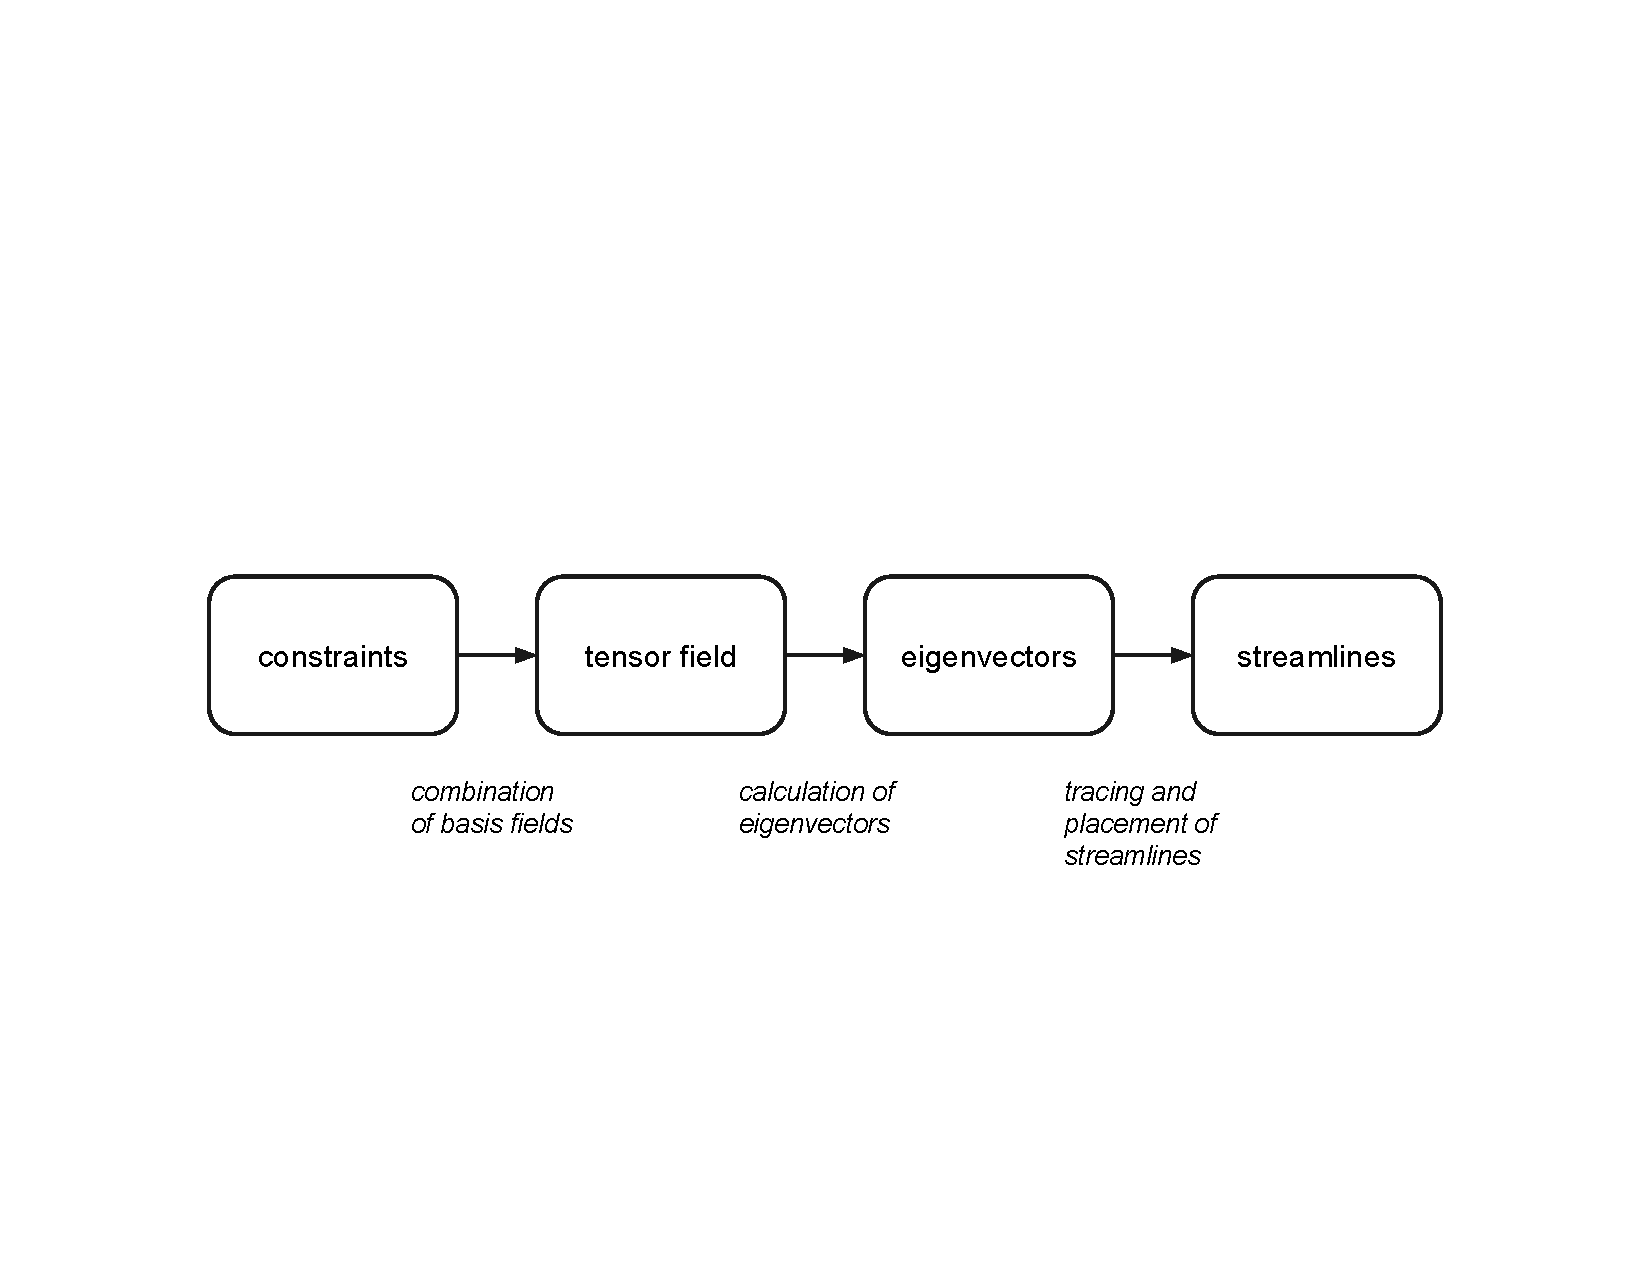
\includegraphics[width=5.5in]{images/pipeline.pdf}
\end{center}
\caption{Overview of our pipeline}
\label{fig:pipeline}
\end{figure*}

\subsection{User-Generated Constraints}
We begin with a JSON parser, which accepts linear and radial constraints.
Constraints must be input with their type, linear or radial, in addition to
their position in the domain (in the form of $x$ and $y$ coordinates), and
finally, if the constraint is linear, it’s direction in radians and magnitude.
In addition, the executable will accept width and height parameters
representing the size of the domain to build street maps on. Together, the JSON
constraints and width/height parameters form the initial input data that will
next be used to form tensor fields.

\subsection{Tensor Field Generation}
From each constraint, a tensor field is defined across the entire domain; this
is called a basis field. The basis fields are then combined to produce a tensor
field that describes the space and takes into account all of the specified
constraints. This is done using an exponential decay combinator, such that when
a basis is combined with others, the constraint that defined it has less
influence on the direction of the field the further a point is from it. The
equations in this section follow closely the system detailed in \cite{chen}.

\paragraph{Linear Constraints}
A linear constraint produces the grid pattern that is a common basis for many
cities (consider the streets of Manhattan). The constraint has two parts: a
magnitude $l$ and a direction $\theta$. The basis field for a linear constraint
is defined as
\[
    T(\pt) =
        l\sqmat{\cos{2\theta}}{\sin{2\theta}}{\sin{2\theta}}{-\cos{2\theta}}
\]
for any point $\bf p$ in the field. It is apparent from this definition that
the direction of a linear basis field is constant, regardless of the value of
$\bf p$.

\paragraph{Radial Constraints}
A radial constraint is used to describe specifically circular areas, such as
roundabouts or more generally curved roads, common in suburban areas. They are
defined at a point $(x_0,y_0)$; major streamlines are drawn as concentric
circles
around the point, while minor ones emanate outwards. The basis field for a
radial constraint at a point $\pt=x_p,y_p$ is defined as
\[
    T(\pt) = \sqmat{y^2-x^2}{-2xy}{-2xy}{-(y^2-x^2)}
\]
where $x=x_p-x_0$ and $y=x_p-x_0$.

\paragraph{Combining Basis Fields}
In order to define a tensor field based on multiple basis fields, we use a
function which sums the basis fields together with an exponential falloff,
so the tensor field is most strongly influenced by a basis field close to
the point around which that basis field is defined:
\[
    T(\pt) = \sum_i e^{-d||\pt-\pt_i||^2}T_i(\pt)
\]
where $d$ is a decay constant, $\pt_i$ is the point at which the $i$th
constraint is defined, and $T_i$ is the basis field corresponding to the $i$th
constraint.

\subsection{Eigenvectors}
The eigenvalues of a tensor $t$ represented by the matrix $\sqmat{a}{b}{b}{-a}$
are:
\[
    \lambda = \pm\sqrt{a^2+b^2} \\
\]
The major eigenvalue, $\lambda_1$, is the larger value, and the minor
eigenvalue, $\lambda_2$ is the smaller value. The corresponding eigenvectors
are then
\[
    \epsilon_i = \left\{1,\frac{\lambda_i-a}{b}\right\}
\]
The eigenvectors are defined if the tensor field is not degenerate (that is,
$a$ and $b$ are both zero) at that point \cite{find-evs}.

\subsection{Streamline Tracing}
Mathematically, the basic streamline tracing algorithm is fairly simple,
however, in order to produce a set of streamlines that approximate a road map,
there are several important cases to consider. In order to trace the
streamlines, we are forced to use a heuristic, since it isn’t possible to trace
a continuous line over a constantly-changing tensor field. In order to
approximate this, we choose a step size $d_\textrm{step}$. Beginning at a seed
point, which is chosen using the methods detailed in section XX, we calculate
the eigenvector at that point, extend a line in that direction with length
$d_\textrm{step}$, and check if we have reached an end condition.  This process
is repeated until the line until one of three end conditions is reached:
\begin{enumerate}
    \item The point is outside the bounds of the map area
    \item The point is within a certain distance of an existing streamline.
    \item The point is part of a cycle
\end{enumerate}

The first is self-explanatory; if the streamline leaves the boundary of the
map, then we don’t need to draw it any more. The second is one of the
alterations we used, based on the work of \cite{chen}. When designing a set of
roads, it is rare that two streets will approach each other and not connect,
whether they approach at a larger angle (an intersection) or are running mostly
parallel to each other (a merge zone). To approximate this, at each point we
find the nearest neighbor out of the streamlines that have already been drawn.
If it is within a certain separation distance, we draw a line directly between
the two points.


\begin{figure*}[t!]
    \todo{image of that nice circular constraint that worked really well with this}
\caption{Haskell implementation of eigenvector calculation}
% \label{fig:cycles} name?
\end{figure*}

The third condition arises mainly with radial constraints. Although a true
hyperstreamline would form a perfect circle around a point, our step-size
approximation means that the trace is more likely to form a spiral. This is
obviously a behavior that would not appear in normal maps (other than an
apocalyptic Boston, perhaps). So, when we detect a streamline circling in on
itself, we close the gap and end the spiral.

\floatstyle{plain}
\restylefloat{figure}
\begin{figure*}[t!]
    \centering
    \begin{subfigure}[b]{2.4in}
        \fbox{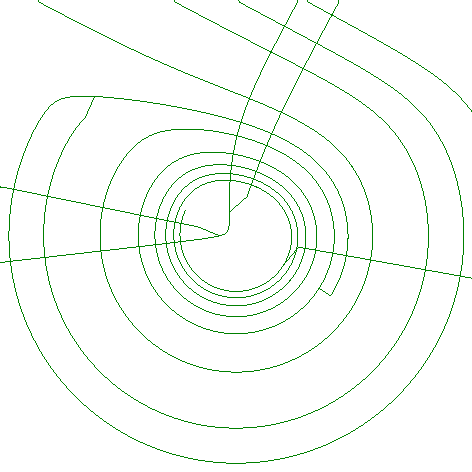
\includegraphics[width=\textwidth]{images/cycle_nodetection.pdf}}
        \caption{without cycle detection}
    \end{subfigure}
    \hspace{20pt}
    \begin{subfigure}[b]{2.4in}
        \fbox{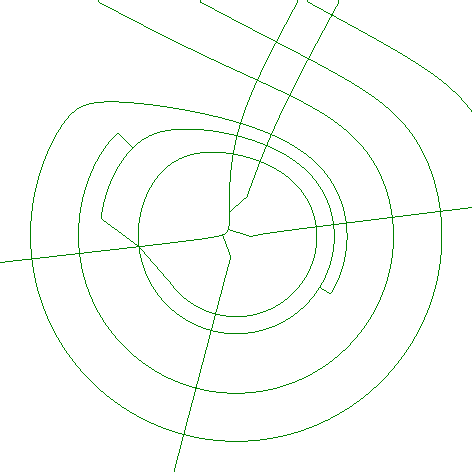
\includegraphics[width=\textwidth]{images/cycle_detection.pdf}}
        \caption{with cycle detection}
    \end{subfigure}
\caption{Streamline tracing cycle detection}
\label{fig:cycles}
\end{figure*}
\floatstyle{boxed}
\restylefloat{figure}

\subsection{Seed Placement}
To begin constructing a streamline, one must choose a seed point—an initial
coordinate in 2D space from which the streamline is traced. In practice, the
matter of carefully choosing seed points is very important in generating an
evenly spaced configuration of roads. We investigated three methods of placing
seed points:
\begin{enumerate}
    \item Random
    \item Furthest-Point
    \item Even Streamline Spacing
\end{enumerate}
Purely random placement of seed points generally results in both clusters of
roads which are too close together and large gaps between roads. In the
furthest-point placement, we place each new seed point within the bounds of the
space such that the distance to all existing streamlines is maximized. As a
simplifying heuristic for this method, we generate a number of random candidate
seed points which is small compared to the infinite number of possible seed
points (constrained only by floating point precision) and choose the one
furthest from all existing streamlines. In practice, this offers a significant
improvement over the random seed placement, and results in a more even
distribution of streamlines.

However, even choosing well-spaced seed points will not necessarily result in
an even distribution of streamlines, since two well-spaced seed points can
result in two streamlines which quickly converge. Therefore, we introduce a
third method. To assess how evenly spaced a set of streamlines is, we will
generate a set of discrete points evenly spaced along each streamline, place
these points into $n\times n$ equal-sized buckets covering the bounds of the
space, and perform a chi-squared goodness of fit test on distribution of points
across bucket, where the expected distribution is uniform:
\[
    \chi^2 = \sum_{i=1}^{n^2} \frac{(O_i-E_i)^2}{E_i}
\]
where $n$ is the number of buckets along each axis, $O_i$ is the observed
number of points in the $i$th bucket, and $E_i=\frac{m}{n^2}$ is the
expected number of points in each bucket, assuming a uniform distribution,
where $m$ is the total number of points in the space.

We will choose the seed point whose corresponding streamline, when added to the
existing set of streamlines, optimizes the evenness of streamline placement,
according to the above metric. As with the previous method, we employ a
simplifying heuristic, generating a relatively small set of candidate seed
points, tracing a streamline from each, determining which streamline results in
a more even field of streamlines, and adding it.

\section{Assessment}
There were two main goals that we set out to achieve with this project. Here we
present a mostly heuristic, slightly quantitative attempt to qualify our
success, using both internal evaluation and comparisons to existing systems
\cite{chen}.

\begin{figure*}[t!]
\begin{verbatim}
-- returns a tuple of the (larger, smaller) eigenvectors of a tensor
eigenvalues :: Tensor -> (Float, Float)
eigenvalues (Tensor a b d) =
  let eval = sqrt (a*a + b*b)
  in  (eval, (-1)*eval)

-- returns a tuple of the (major, minor) eigenvectors for a tensor
eigenvectors :: Tensor -> (V2.Vector2, V2.Vector2)
eigenvectors (Tensor a 0.0 d) =
  if a > d then (V2.Vector2 1 0, V2.Vector2 0 1)
     else (V2.Vector2 0 1, V2.Vector2 1 0)
     eigenvectors (Tensor a b d) =
       let (eval1, eval2) = eigenvalues (Tensor a b d)
           mkEvec eval    = V2.Vector2 1 ((eval - a) / b)
       in (mkEvec eval1, mkEvec eval2)
\end{verbatim}
\caption{Haskell implementation of eigenvector calculation}
\label{fig:evecs}
\end{figure*}

\subsection{Modularity \& Extensibility}
We believe that we were successful in creating a modular system with reusable
parts that is easy to understand, extend, and modify. One way to illustrate
this is by looking at our pipeline. As a refresher, look at Fig. ***. Each
step of the pipeline has a clear correspondence in the modules that we have
written. We have two modules to deal with constraints, \texttt{Constraint}. To
transform
constraints to maps, we have written \texttt{TensorField} and \texttt{Tensor}
modules, the latter
of which performs operations on tensors including eigenvector calculations, as
well as \texttt{Streamline}, which has the ability to calculate seed points
and trace
lines.

We also created several generally useful modules, including \texttt{Vector2},
which performs basic operations on 2-dimensional vectors and
\texttt{NearestNeighbor}, which defines a type class for a structure that can
store \texttt{Vector2}s and query for the nearest neighbor, as well as a
bucket-based implementation of such a data structure. To deal with input and
output, we created a \texttt{JSONParser} so that our input can come from any
source that is capable of producing JSON, and an \texttt{SVGWriter}, which
deals with the widely-used file format that produces the output seen in many of
the figures in this paper.

In an attempt to compare this with the original work, we consulted the header
files available with Chen’s code. The system has significantly more
functionality than ours, but we had some difficulty discerning which modules
were parallel to ours. The \texttt{tensoranalysis} contains methods for tensor
line tracing, and \texttt{ClosedStreamlineTracing} seems to be related,
although we did not find documentation on the difference between open and
closed tracing. \texttt{SeedPointCtrlDlg} is a dialogue probably related to the
OpenGL framework, but didn’t have the actual calculations of seed points. At
the least, our implementation has a more direct pipeline-to-module correlation,
which will be beneficial for future contributors who wish to build off of our
work.

\subsection{Natural Expression of Underlying Mathematics}
Overall, this seemed to be successful. In general, functional languages are
well suited to express mathematics. Our decision to implement this program in
Haskell meant that that we were able to take advantage of this natural
proclivity towards math in order to make our code easy to understand.

An example of this can be seen in the calculation of eigenvectors. We derived
the formula for the eigenvector of a symmetric, traceless tensor
(see Section~\ref{sec:math}) and implemented it in the functions in
Figure~\ref{fig:evecs}.

In [Chen], there is a 75-line function,
\texttt{cal\_eigenvecs\_onevert\_quad}, to do approximately the same thing. There
is a fair amount of documentation in the body of the function, explaining what
each line does, but there also seem to be some side effects relating to global
variables and large data structures that the authors found difficult to follow,
mostly by the nature of the language.  Generally speaking, we found that the
mathematics was significantly easier to express and review in a Haskell
implementation.

\section{Conclusion}
In this paper we have presented the underlying mathematics and functional
implementation of the work described in \cite{chen}, with the goals being that a
functional implementation would easily express the mathematics and provide
modularity that the imperative implementation provide in \cite{chen} could not.


\bibliographystyle{alpha}
\bibliography{references}

\end{document}
